\chapter{Структура Cloud Firestore}
\label{cha:appendix1}

\begin{figure}[h]
	\centering
	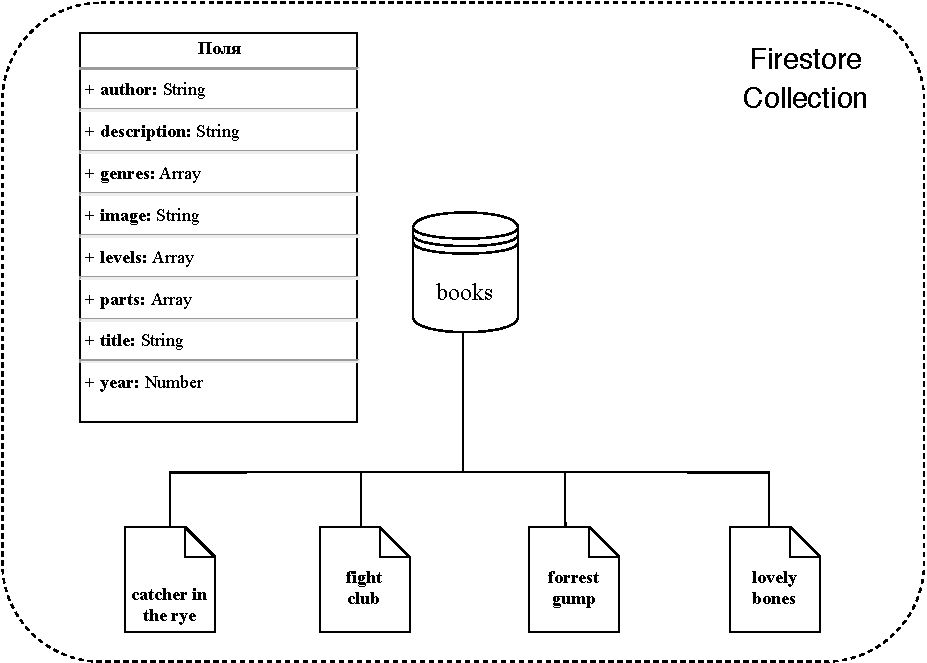
\includegraphics[width=\textwidth, keepaspectratio]{figures/books}
	\caption{Структура коллекции books}
	\label{fig:booksDiagram}
\end{figure}

\begin{figure}[h]
	\centering
	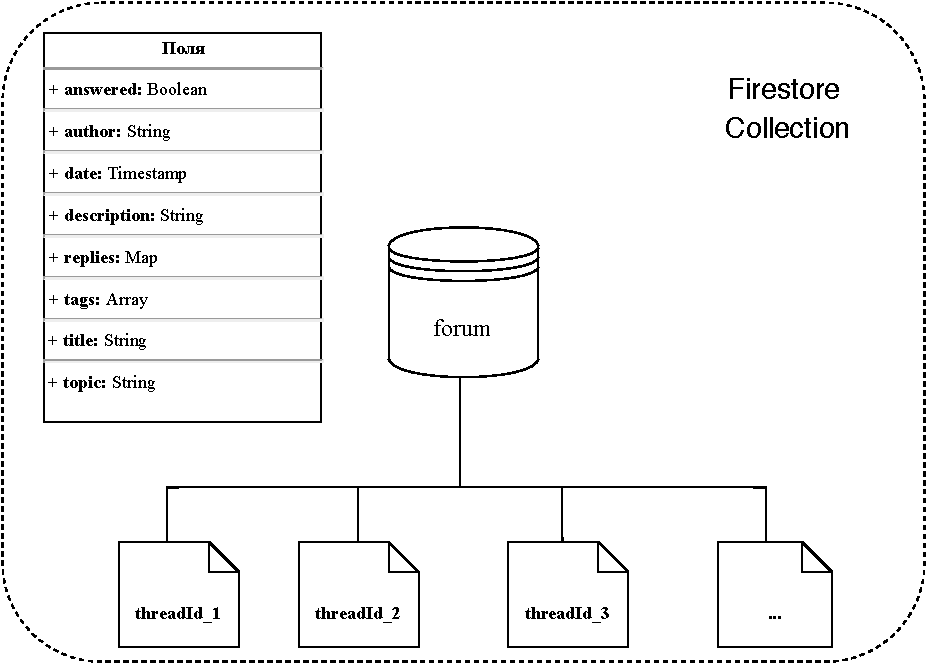
\includegraphics[width=\textwidth, keepaspectratio]{figures/forum}
	\caption{Структура коллекции forum}
	\label{fig:forumDiagram}
\end{figure}

\begin{figure}[h]
	\centering
	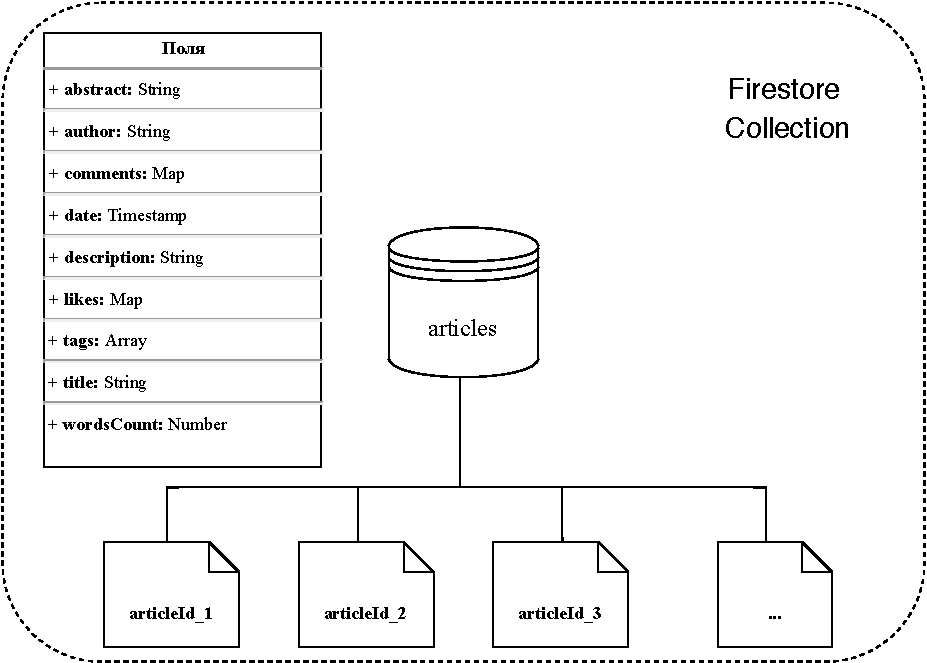
\includegraphics[width=\textwidth, keepaspectratio]{figures/articles}
	\caption{Структура коллекции articles}
	\label{fig:articlesDiagram}
\end{figure}

\begin{figure}[h]
	\centering
	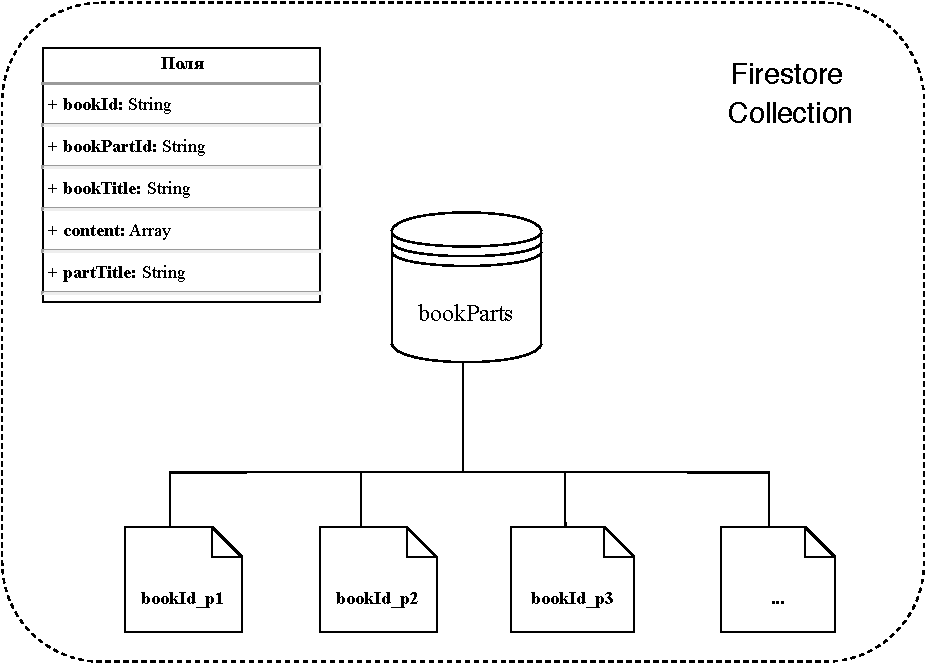
\includegraphics[width=\textwidth, keepaspectratio]{figures/bookpart}
	\caption{Структура коллекции bookParts}
	\label{fig:bookPartsDiagram}
\end{figure}

\begin{figure}[h]
	\centering
	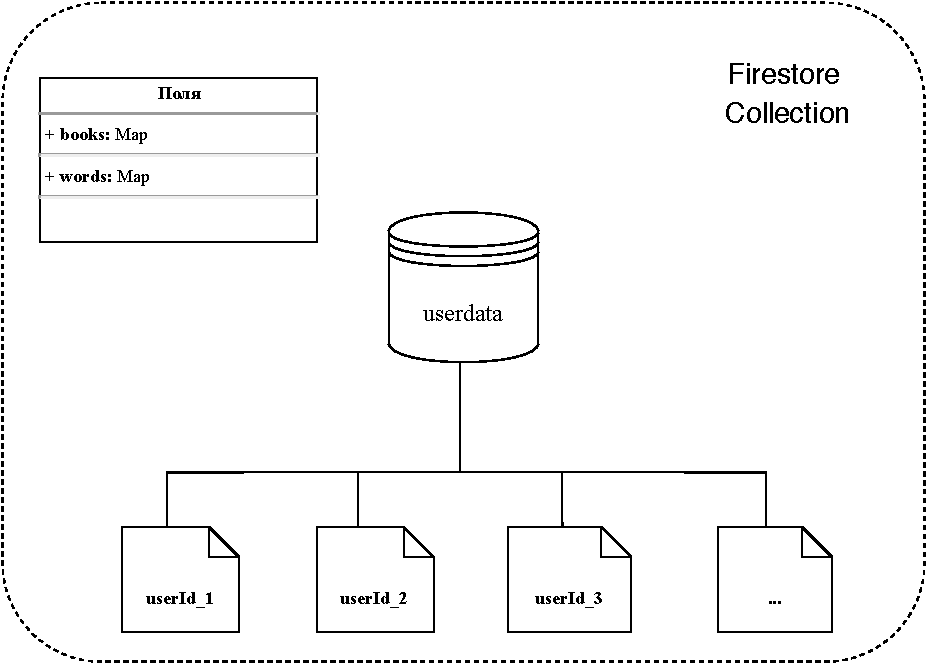
\includegraphics[width=\textwidth, keepaspectratio]{figures/userdata}
	\caption{Структура коллекции userdata}
	\label{fig:userdataDiagram}
\end{figure}

\begin{figure}[h]
	\centering
	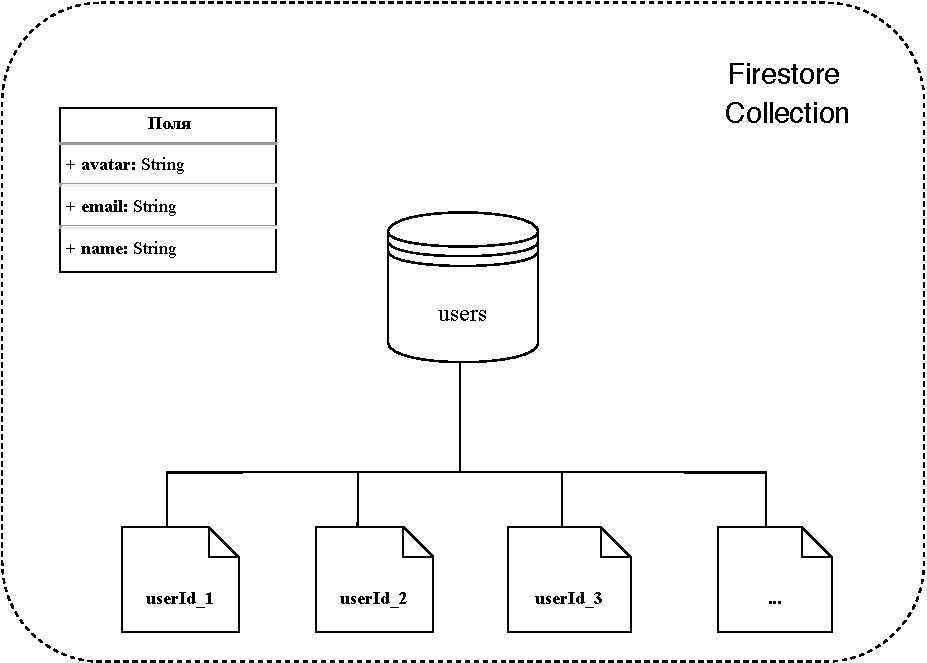
\includegraphics[width=\textwidth, keepaspectratio]{figures/users}
	\caption{Структура коллекции users}
	\label{fig:usersDiagram}
\end{figure}

%%% Local Variables: 
%%% mode: latex
%%% TeX-master: "rpz"
%%% End: 
